% !TeX spellcheck = en_US
\chapter{Approach}\label{ch:approach}

This chapter contains the solution approaches to the parts of the thesis. Firstly, a formal model of a compressor is defined. Based on that, the key performance indicators which will be used to measure the performance of the single compressors are introduced.

Secondly, the two existing compressors HDT and GRP are compared.

Finally, improvements of the compression will be suggested.


\section{Compressor Models}

Here, two compressor models will be introduced, one for general compressor and another one for RDF compressors. 

\subsection{General Compressor Model}\label{sec:generalcompressorModel}

A general purpose compressor $C$ can be described as follows: $C$ takes an input $in$ and produces an output. That step is called compression. Decompression can be described as tasking $out$ as an input and producing $in$.

\begin{figure}
	\centering
	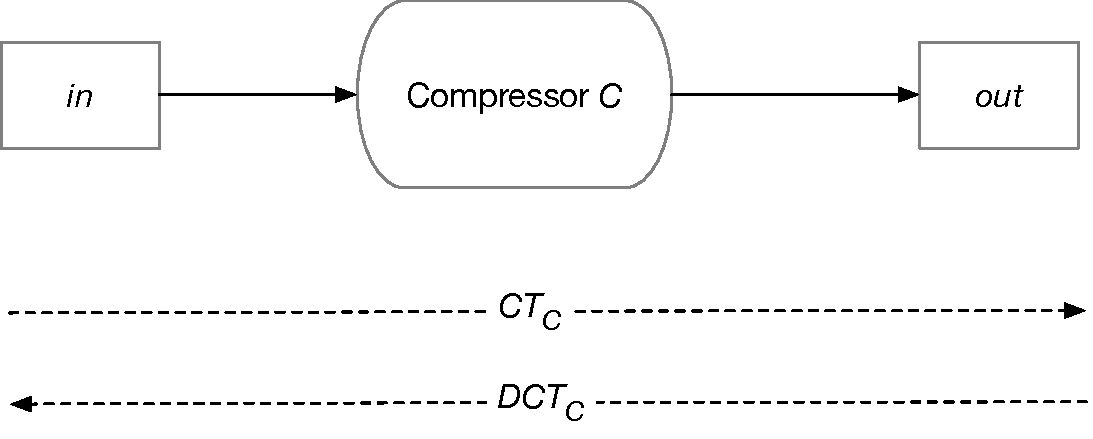
\includegraphics[width=0.8\linewidth]{figures/approach/model_general}
	\caption{Visualization of the General Compressor Model.}
	\label{fig:generalcompressorModel}
\end{figure}

\subsection{RDF Compressor Model}\label{sec:compressorModel}

This section introduces a formal model for an RDF compressor which can be seen as a sub class or extension of the general model in Ch.~\ref{sec:generalcompressorModel}. It is illustrated in Fig.~\ref{fig:compressorModel}. Here, the compressor $C$ is more complex as it consists of two components. The first one is called $Dict_C$ and it handles the dictionary compression. That mechanism has already been introduced in the context of HDT (see~Ch.~\ref{related_work_hdt}). It assigns an ID to each URI, literal or blank node ID of the graph and can then also further compress the dictionary (like in HDT with prefix trees). The result of $Dict_C$ is $out_{dict}$ which is displayed in the right of Fig.~\ref{fig:compressorModel}. 

The IDs created by $Dict_C$ are then delivered to the second component $Graph_C$ which is responsible for compressing the RDF graph. It only uses the IDs from $Dict_C$ and does not know about the URIs, literals and blank node IDs. Its result is called $out_{graph}$ which, together with $out_{dict}$, forms the complete output $out$. $out_{graph}$ and $out_{dict}$ can each be a single file or set of files. 

\begin{figure}
	\centering
	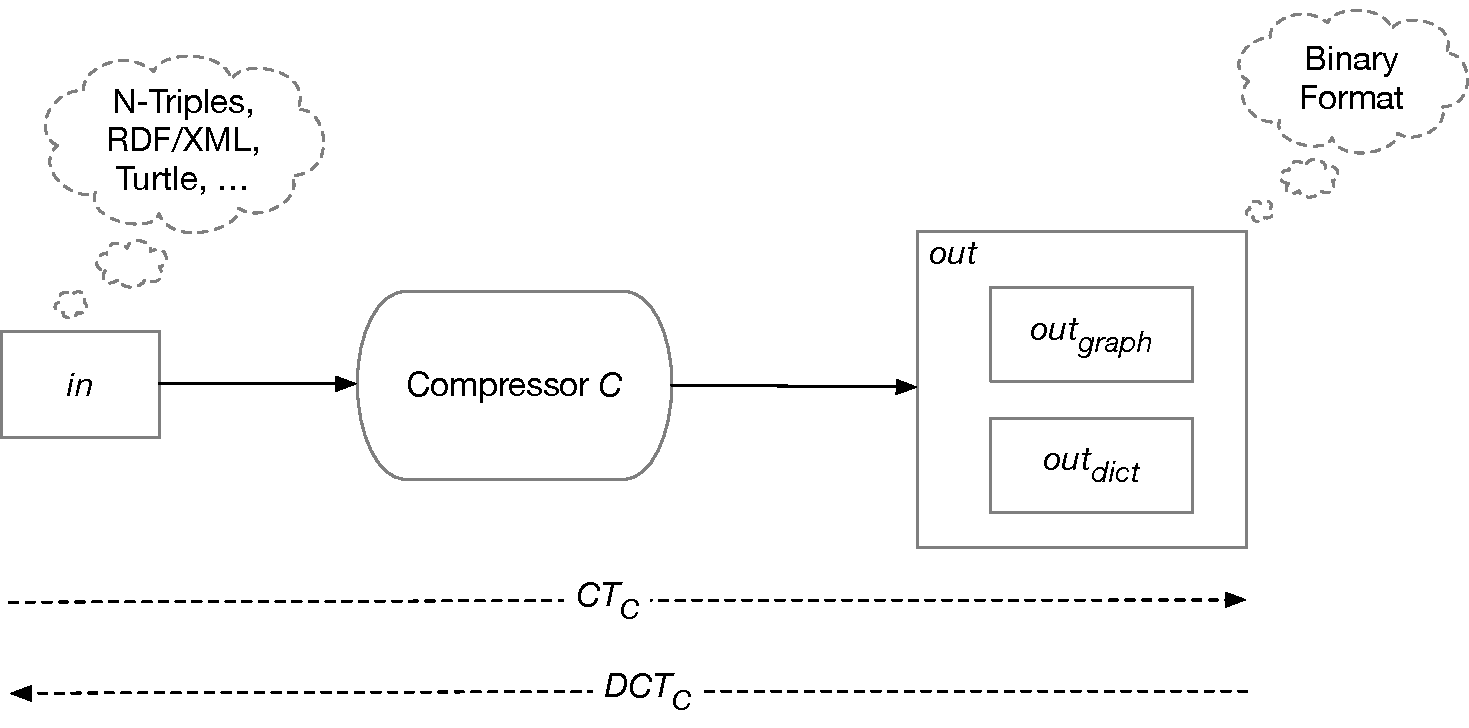
\includegraphics[width=\linewidth]{figures/approach/model}
	\caption{Visualization of the RDF Compressor Model.}
	\label{fig:compressorModel}
\end{figure}


\subsection{Existing RDF  Compressors}

Table~\ref{tab:compressorsOverview} shows an overview of the RDF compressors discussed in this thesis and in which way they fulfill the model. As already explained in Ch.~\ref{related_work_hdt}, $Dict_{HDT}$ assigns IDs and compresses the dictionary. In contrast, $Dict_{GRP}$  only assigns IDs and omits the dictionary afterwards. $Dict_{GRP}$ is therefore not a real dictionary compressor. We solve this problem by letting GRP use $Dict_{HDT}$. This way, comparing HDT and GRP in a fair way is possible.

\begin{center}
	\begin{tabular}{|c|c|c|}
		\hline 
		& $Dict_{C}$ & $Graph_{C}$ \\ 
		\hline \hline
		HDT & $\checkmark$ & $\checkmark$  \\ 
		\hline 
		GRP & only ID assignment (no compression or storage of dictionary) & $\checkmark$ \\ 
		\hline 
	\end{tabular} 
	\captionof{table}{Overview of RDF compressors presented in this thesis.}	
	\label{tab:compressorsOverview}
\end{center}

\section{Key Performance Indicators}

In the following two sections, key performance indicators for general and RDF compressors are introduced. Those indicators will be measured in to determine the overall performance for the different compressors.

\subsection{Compression Ratio}

One of the key performance indicators for a compressor $C$ is its compression ratio. Let $m$ be a single file or a set of files. Then $|m|$ is defined as the size which is measured in bytes. The compression ratio is defined by the following equations:

\begin{align}
CR_{C} = \dfrac{|out|}{ |in|} \label{eq:complete}
\end{align}

\begin{align}
CR_{Dict_C} = \dfrac{|out_{dict}|}{ |in|} \label{eq:dict}
\end{align}

\begin{align}
CR_{Graph_C} = \dfrac{|out_{graph}|}{ |in|} \label{eq:graph}
\end{align}

Eq.~\ref{eq:complete} defines the compression ratio for the whole output $out$. Therefore, it is applicable to general and RDF compressors.

In contrast, Eq.~\ref{eq:dict} and~\ref{eq:graph} define the compression ratio only with regard to $out_{dict}$ and $out_{graph}$, respectively. They are only applicable for RDF compressors, since a general compressor has no distinction between $out_{dict}$ and $out_{graph}$. In some cases it is of interest to only consider either dictionary or graph compression.

Sometimes $CR$ is used instead of $CR_C$ if it is clear from the context, which compressor $C$ is considered.

If $C$ is an RDF compressor, then $CR_C$ is not always measured with respect to the whole output $out$, but sometimes only with respect to $out_{graph} \text{ or } out_{dict}$. This is due to the fact that in some cases it is interesting to only consider the compression of the dictionary or the graph.

As shown in Fig.~\ref{fig:compressorModel}, $in$ can have different formats. That has to be taken into account with regard to $CR$ as those formats implicate different input sizes. When $CR$ of two compressors is compared, their input has to have the same format.

\subsection{(De-)Compression Time}

Another key performance indicator of a compressor $C$ is its compression time ($CT_C$) and decompression time ($DCT_C$). These metrics also depends on the input data and indicate the run time needed for compression and decompression of the data, respectively. The run time is typically measured in milliseconds. $CT_C$ and $DCT_C$ are also shown in Fig.~\ref{fig:generalcompressorModel} and~\ref{fig:compressorModel}. They are defined the same for general compressors and RDF compressors. Furthermore, $CT_C$ and $DCT_C$ are only measured for the whole compressor $C$, not for $Dict_C$ or $Graph_C$.

Analogously to $CR$, if is clear from the context which compressor is considered, $CT$ and $DCT$ are used instead of $CT_C$ and $DCT_C$, respectively.


\section{GRP vs HDT}\label{sec:approachGRPvsHDT}

In this section, the two existing compressors - HDT and GRP - will be compared. Therefore, the features of the compressors and their applicability to certain properties of RDF graphs are discussed.

The question is whether there are certain properties/features that an RDF graph can have, and which have a positive or negative impact on the compression ratio of one or both algorithms. 

As HDT and GRP use the same method for compressing the dictionary ($Dict_{HDT}$), we only compare $Graph_{HDT}$ and $Graph_{GRP}$ in this chapter.

\subsection{Relation Between Structure of Data and Compression Ratio}\label{sec:relationDataStructureComprRatio}

First these features are considered for HDT. Fig.~\ref{fig:hdt_overview_1} is shown again. There, it is noticeable that the size of the data becomes smaller if there are only a few subjects. This is the case because the bit-array $B_p$ contains a 1 every time a new subject is considered. For example, if there is only one subject, then $B_p$ consists only of zeros.\todo{stimmt anscheinend nicht}

\begin{figure}[h]
	\centering
	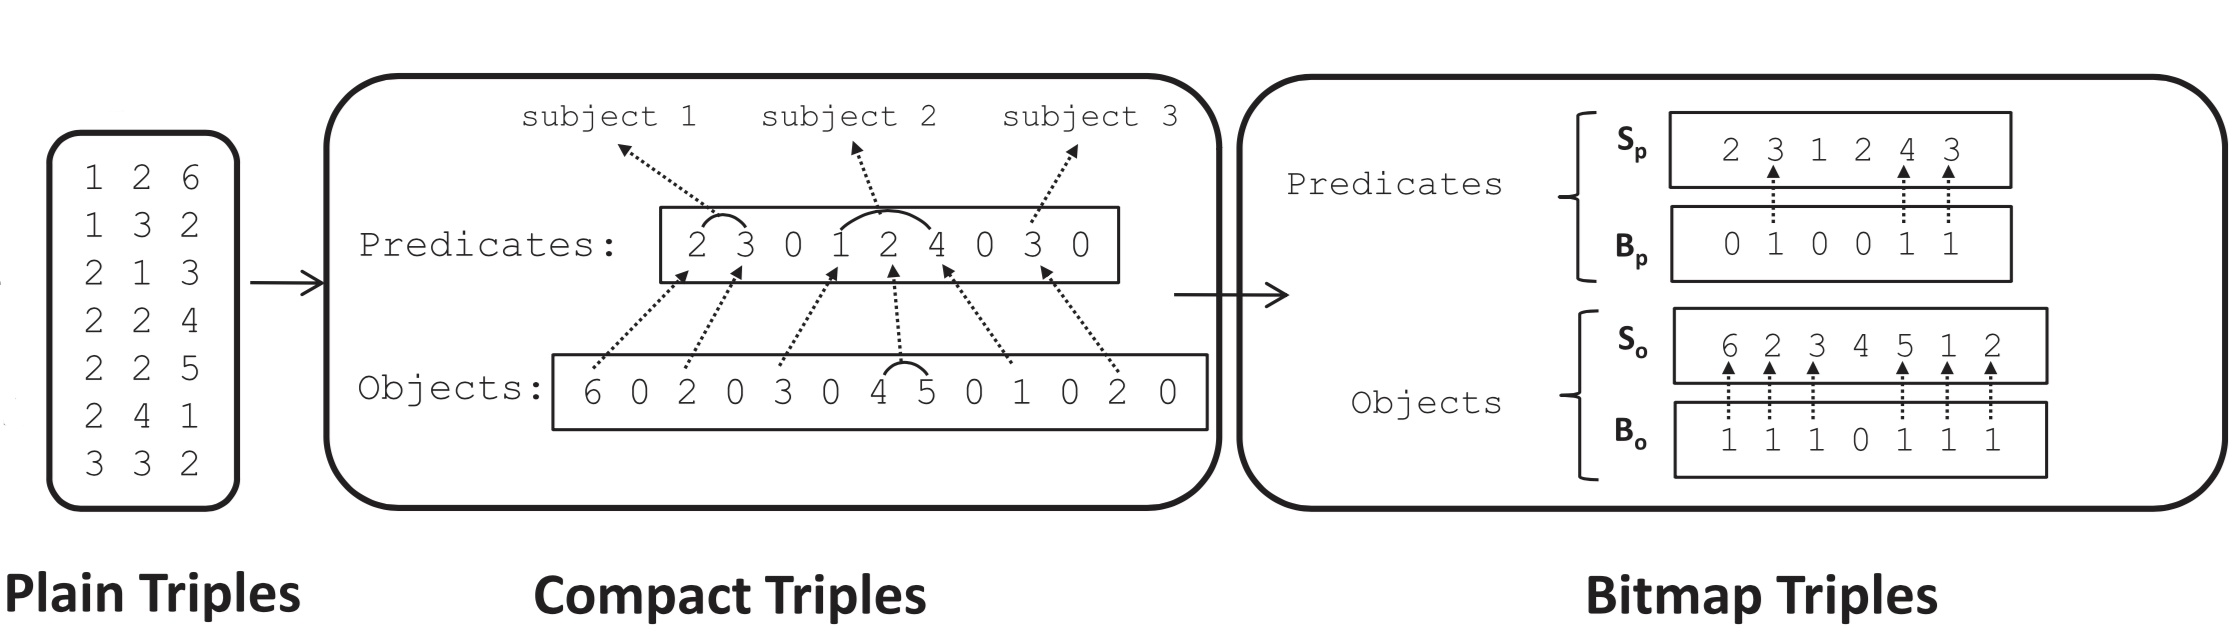
\includegraphics[width=1\textwidth]{figures/relatedwork/hdt1}
	\caption{Three different representations of triples in HDT, figure from~\cite{hdt}.}
	\label{fig:hdt_overview_1}
\end{figure}

For GRP that feature analysis is more complex. Since GRP constructs grammar rules by using the graph's structure, it can make use of sub graphs that are much more complex than the star pattern HDT is using. There can be many features that can lead to different constructible grammar rules. Those will not be discussed here, as these pattern can become arbitrarily complex, because they can be nested among each other. But one insight is that GRP's compression ratio will be bigger when there are more different predicates in the graph. This is true, because GRP's grammar rules are based on repeating patterns and, hence, repeating edge labels as part of these patterns.

\subsection{Dictionary Size}

\todo{gucken ob sectoin nötig,passt nicht mehr}

As already explained in Ch.~\ref{ch:related_work}, HDT divides an RDF file into its header, dictionary and triples component. This is partially also true for GRP except that GRP does not create a header. But it also assigns an ID to every URI or literal and then only works with these IDs. Unfortunately the authors of~\cite{maneth} did not work on efficient storing of the dictionary. In GRP the size for the dictionary component is just ignored. Therefore we have to add this size in order to compare GRP with HDT in a fair way. To achieve that we just add the same size to the compressed size of GRP that HDT would need to store the dictionary.


\section{Compression Improvements}\label{sec:approachComprRatioImprovements}

First comparisons of $Graph_{HDT}$ and $Graph_{GRP}$ (see~Ch.~\ref{sec:evaluationHDTvsGRP}) showed that  $Graph_{GRP}$ achieves a better compression ratio. Therefore, Ch.~\ref{sec:approachOntKnowledge} will mainly focus on improving $Graph_{GRP}$. But Ch.~\ref{sec:approachDictImprovements} is about the improvement of $Dict_{HDT}$ which is used for both HDT and GRP.



\subsection{Ontology Knowledge}\label{sec:approachOntKnowledge}

As already discussed in Ch.~\ref{sec:relatedworkOntology}, an ontology contains meta data about an RDF graph.

This chapter will investigate whether it is possible to change the structure of an RDF graph by applying knowledge from its ontology so that it is better compressible for GRP, but at the same time remains semantically equivalent to the original graph. In this way no data would be lost after the compression.

In Ch.~\ref{sec:relationDataStructureComprRatio} it has already been mentioned that GRP makes use of much more complex sub structures than HDT. It will therefore be interesting to see how applying ontology knowledge influences GRP's compression ratio.

This chapter is about elaborating the theoretical concepts of OWL and investigating how they can be used for grammar-based compression.

Let \[ elr = \dfrac{\text{number of different edge labels}}{\text{number of edges}} \] (edge label ratio) be the ratio of the edge labels or properties to the total number of edges of the graph. 

Generally it can be said that GRP can compress a graph better if $elr$ is lower, because then there it is more likely that there is much redundancy in the graph. However, if the graph structure becomes unfavorable for GRP, the compression ratio may still be worse at a lower value for $elr$.


\subsubsection{Symmetric Properties}

\todo{besseres Bsp}

There is a class in~\cite{owl} called {\tt owl:SymmetricProperty}~\footnote{The prefix {\tt owl:} is used for every entity in the context of OWL.} which expresses that a certain other predicate $p$ is symmetric. This means, if there is a triple $(s,p,o)$ in the graph, then there can also be a triple $(o,p,s)$ at the same time. In reality, however, it can happen that only one of the two triples is explicitly mentioned and the second triple is only implicitly present. The idea is to always add the other triple to the graph in such a case. This makes the graph larger at first, but more grammar rules can be found. This is because $elr$ can be reduced by adding it, which can lead to a better compression ratio. At the same time this will not result in an unfavorable structure. The procedure is illustrated in Fig.~\ref{fig:symmetricMat}. That graph shall be seen as a sub graph of a much larger graph. Here the predicate $p$ is symmetric, so the edge from node 3 to 2 was added, $p_1$ is not symmetric. Due to the addition, the digram of Fig.~\ref{fig:symmetricMatDigram} can now be found twice, whereas it was previously found only once. These two occurrences overlap and therefore cannot be applied both. However, it may be that one of the two occurrences cannot be replaced because the nodes involved are still connected to other nodes that are not shown in this figure. So the addition increases the probability that the digram can actually be replaced. At the same time the degree of nodes 2 and 3 is increased by one. But this should not really decrease the chance of finding other digrams in the graph, since 2 and 3 have already been connected before.


\begin{figure}[h]
	\centering
	\subfloat[A sub graph to which the edge from node 3 to 2 was added.]{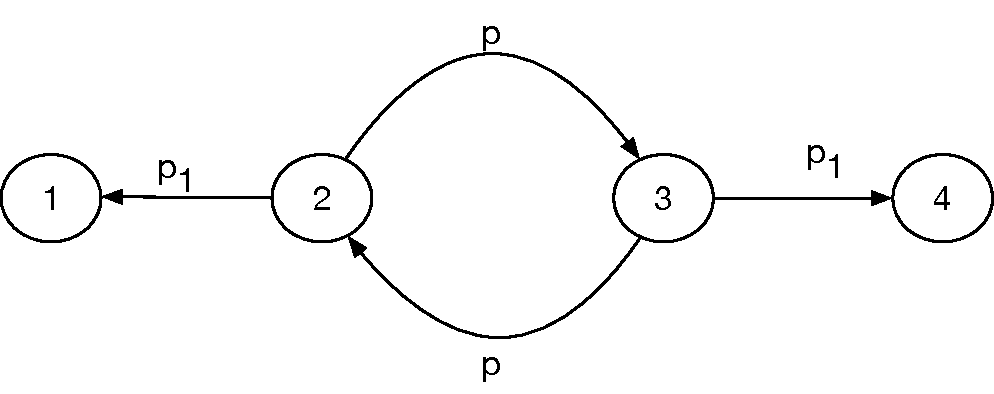
\includegraphics[width=0.45\textwidth]{figures/approach/symmetricMat}\label{fig:symmetricMat}}
	\hfill
	\subfloat[The digram that can be found twice in the graph of Fig.~\ref{fig:symmetricMat}]{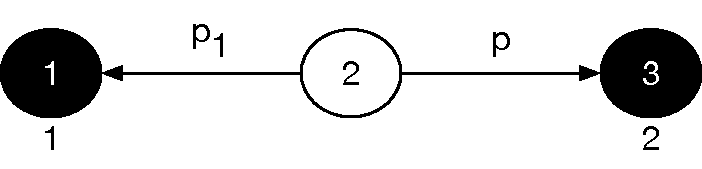
\includegraphics[width=0.45\textwidth]{figures/approach/symmetricMatDigram}\label{fig:symmetricMatDigram}}
	\caption{Visualization of the benefits of adding symmetric edges to the graph. $p$ is symmetric, $p_1$ is not symmetric.}
	\label{}
\end{figure}

\subsubsection{Inverse Properties}

One property of~\cite{owl} is {\tt owl:inverseOf}, which is defined for two properties $p_1, p_2$. If $(s,p_1,o)$ exists then $(o,p_2,s)$ should also exist and vice versa. Analogously to {\tt owl:SymmetricProperty} it can be the case that only one of the two triples is explicitly mentioned. The approach is similar to the symmetric properties. It is reasonable to argue in a similar way for adding those edges to graph here. It can decrease $elr$ if there are many occurrences of a few inverse properties. Also, adding those edges will not really make the graph's structure more complex since all the nodes were already connected before. 


\subsubsection{Transitive Properties}

In~\cite{owl}, a predicate can be denoted as transitive ({\tt owl:TransitiveProperty}). Let $p$ be transitive. If the triples $(1,p,2),(2,p,3)$ exist then $(1,p,3)$ should also exist. Consequently, this holds also for an arbitrarily long path from $1$ to $3$, as illustrated in Fig.~\ref{fig:transitiveMat}. The shown graph shall again be seen as some sub graph. The approach is to remove the triple $(1,p,n)$. This is sensible, as it gives the nodes 1 and $n$ a lower degree, and therefore GRP can have a higher chance to find other digrams in which those nodes are involved (they are not shown in Fig.~\ref{fig:transitiveMat}). A further argument against adding edges is that this would dramatically increase the number of edges, because for each pair $(x,y)$ (with $x,y\in \{1,...,n\} $  and distance between $x$ and $y$ greater than 1), an edge $(x,y)$ would be added. After increasing the graph's size so much it is unlikely that $out_{graph}$ becomes smaller even if more digrams could be found.

\begin{figure}[h]
	\centering
	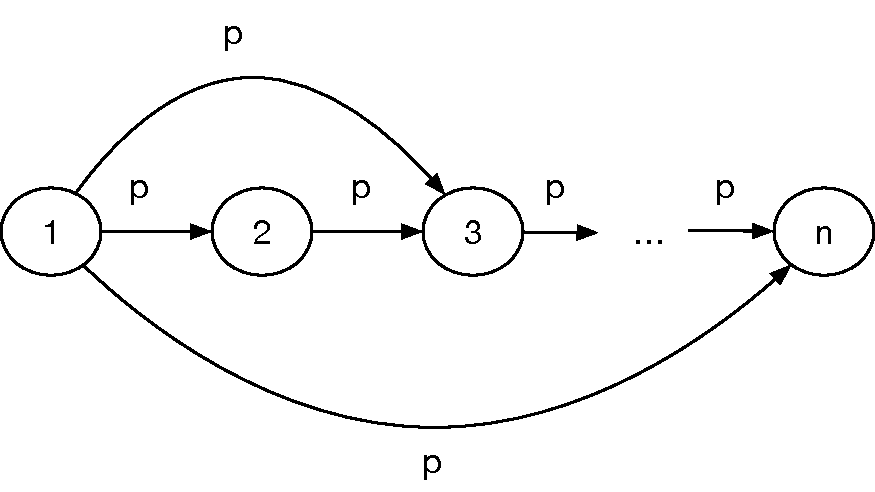
\includegraphics[width=0.6\textwidth]{figures/approach/transitiveMat}
	\caption{A sub graph with the transitive predicate $p$.}
	\label{fig:transitiveMat}
\end{figure}


\subsubsection{Equal Properties}

In OWL there are the predicates {\tt owl:equivalentProperty} and {\tt owl:sameAs}. The first one denotes that two properties are equivalent, but is does not mean that they are equal. In contrast, the latter one is expressing equality. If there is a property $p$ which is equal to other properties $p_1,..,p_n$, then one approach could be to replace each occurrence of $p_1,..,p_n$ with $p$. This would reduce $elr$ and, at the same time, not change the structure of the graph. However, this approach was not implemented, since the thesis focuses on compressing single RDF graphs and {\tt owl:sameAs} typically connects multiple graphs with each other. Compressing multiple graphs would lead to more complexity, because not only properties can be the same but single nodes can be marked as the same as well.


\subsection{Dictionary Improvements}\label{sec:approachDictImprovements}


According to~\cite{hdt}, the dictionary ($out_{dict}$) makes up most of the memory of a compression output. First results in Ch.~\ref{ch:evaluation} also show that. It is therefore worth investigating whether the dictionary can be compressed better. It can be taken advantage of certain features of the dictionary to achieve that. In order to do that we use $Dict_{HDT}$ as the basis and further improve it.

\subsubsection{Literals}\label{sec:approachLiterals}

Objects in RDF can be literals. Literals typically contain constant values and usually have no common prefixes. Therefore the compression of HDT is not suitable for these. It would be possible to use different compression techniques for different types of data values (integer, double, string, etc.). The thesis will focus on compressing strings.

Since those strings can contain whole flow texts, a text compression would probably be well applicable. An example of such a text compression is a Huffman Code~\cite{huffman}. Here, every single character of a text is binary coded, whereby frequently occurring characters get short and rare characters get longer codes. These codes are expressed by a binary Huffman tree. An example can be seen in Fig.~\ref{fig:huffmantree}. Each leaf contains a symbol whereas the ones and zeros on the path to the symbol define its code. The tree is constructed in such a way that paths to frequent characters are shorter than those to rare characters. The whole procedures can be seen in~\cite{huffman}.

\begin{figure}
	\centering
	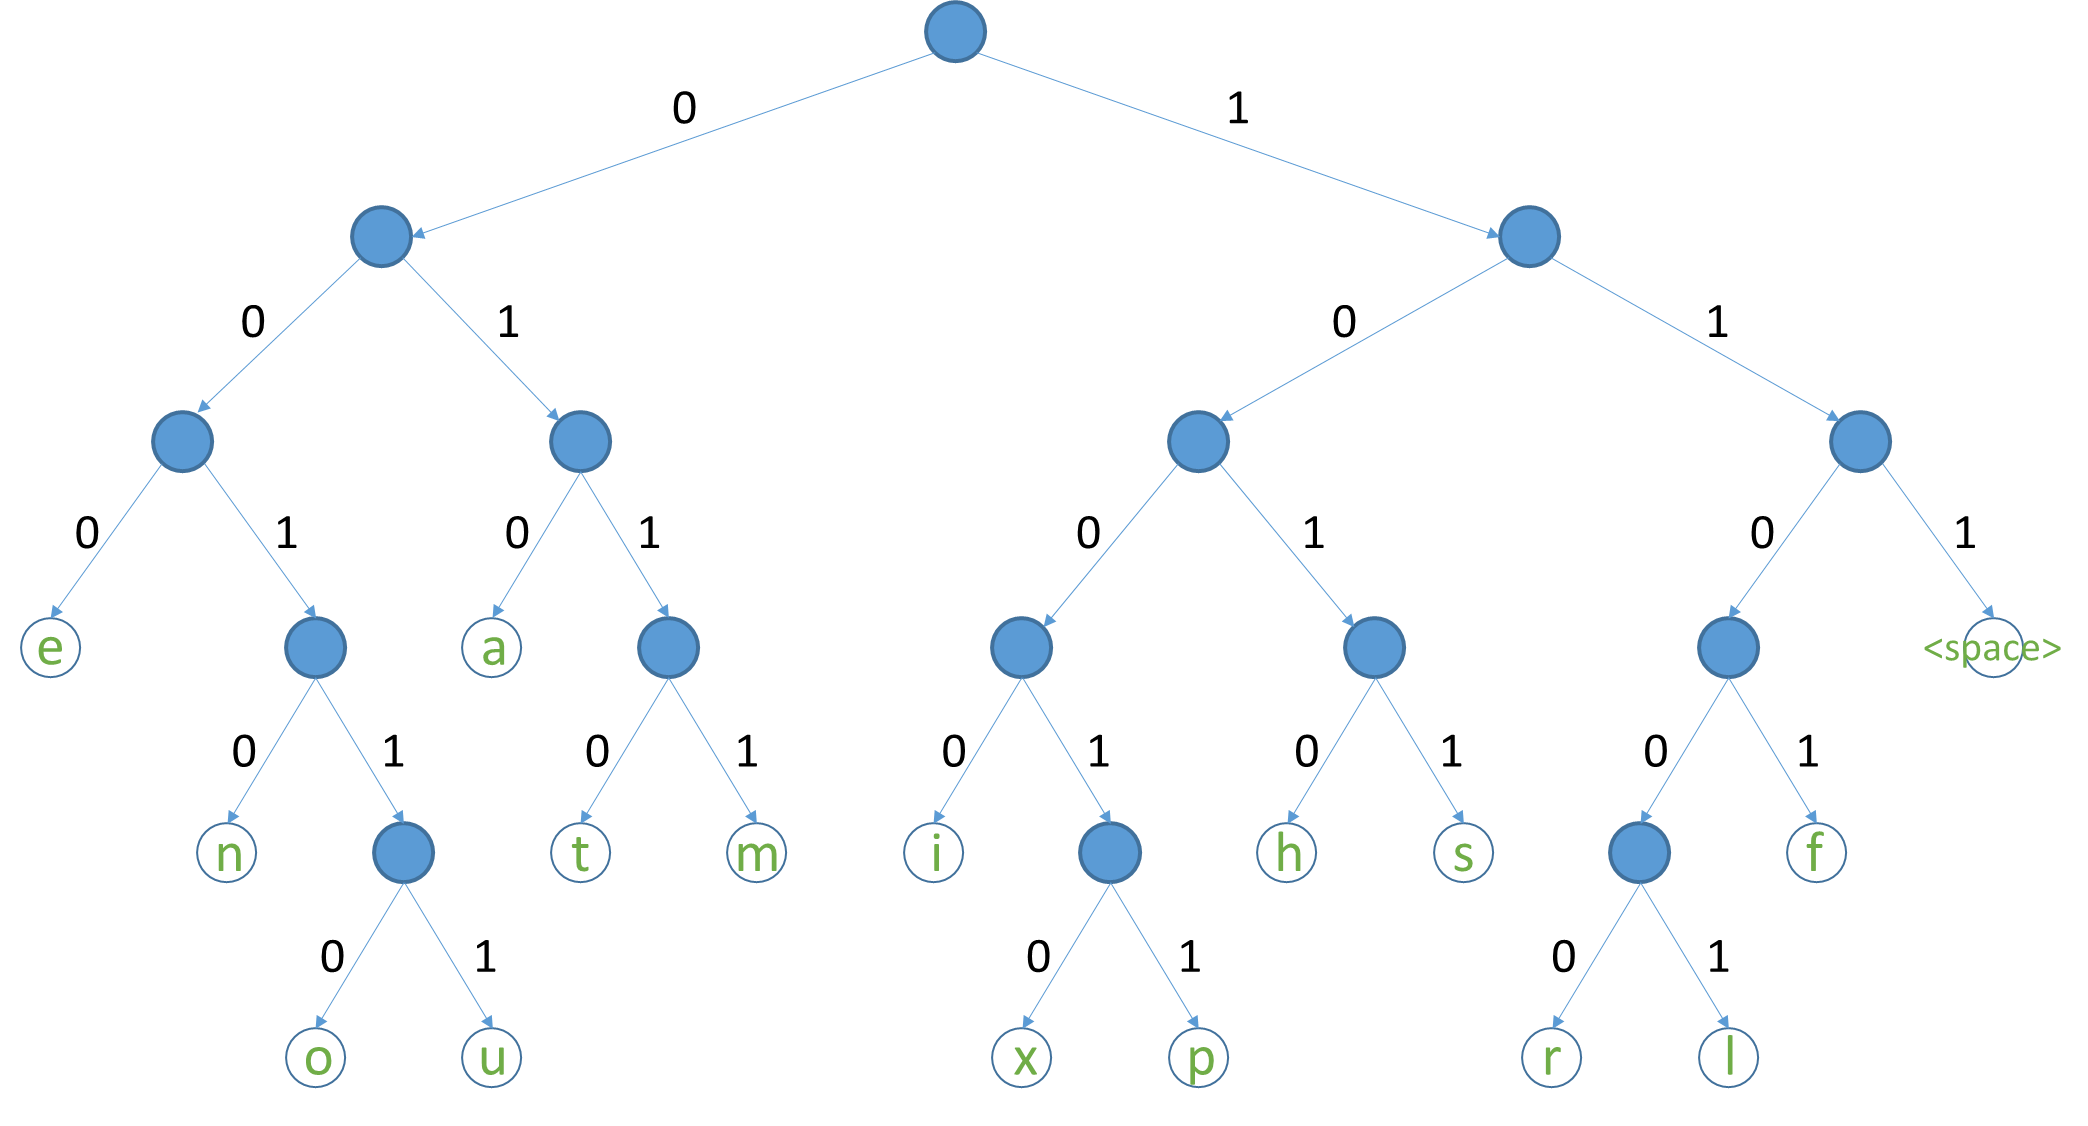
\includegraphics[width=0.9\linewidth]{figures/4_rdf_specific_features/huffman}
	\caption{An example of a Huffman Tree.}
	\label{fig:huffmantree}
\end{figure}

\subsubsection{Blank Nodes}\label{sec:approachBlankNodes}

As already mentioned in Ch.~\ref{sec:relatedworkRDF} every blank node gets an ID. These IDs are usually chosen arbitrarily and have no meaning beyond that. When reading an RDF graph with the Jena-API~\footnote{\label{foot:5}https://jena.apache.org/index.html} (which is used by HDT according to~\cite{hdt}) random long strings are assigned for the blank nodes, which are quite long. They also have no common prefixes, which makes the HDT dictionary compression ineffective here. 

To improve the compression, the IDs of the blank nodes could be reassigned. For example, numbers from 1 to $n$ ($n=$ number of blank nodes) can used to get short IDs. 

Another possibility is not to save the IDs of the blank nodes at all. In HDT all strings in the dictionary (including the blank node IDs) are mapped to short IDs. Thus, the blank node IDs are in principle already stored. They can therefore be removed from the dictionary. HDT must then be changed so that it can handle the case in which it does not find a corresponding string in the dictionary for a certain short ID. At this point it would know directly that the considered node is a blank node and the longer blank node ID is unimportant. Such a situation will occur when a decompression is performed.















